\documentclass[aspectratio = 169]{beamer}
\usetheme{OsloMet}
\setbeamersize{text margin left=0.5cm,text margin right=0.5cm}
\usepackage{style}

\renewcommand{\S}{\mathcal{S}}
\newcommand{\T}{\mathcal{T}}
\author[]{Wenning Wei\\ Mahsa Azizi\\ Erik Chan\\ Xilai Fu\\ S. Parisa Torabi}
\title{Modeling Canadian\protect\\ Heavy Crude\protect\\ Congestion Pricing}


\begin{document}

\begin{frame}{OUTLINE}
\begin{enumerate}
\setlength\itemsep{2em}
    \item\Large{Introduction}
    \item Model
    \item Result
    \item Conclusion
\end{enumerate}
\end{frame}

\section{Introduction}
\begin{frame}{Introduction}
\Large{What effects price benchmark in oil market?}


\begin{itemize}
\setlength\itemsep{2em}
    \item \Large{Crude oil classification (heavy, light)} 
    \item \Large{Location of extraction}
    \item \Large{Transportation capacity}
%%%% Capacitance is not a word that makes sense in this context. This is an electrical engineering term to denote the % ratio of electrical charge.
\end{itemize}
\end{frame}

%Why was this commented out? It was agreed in the meeting that you would talk about this time series.
\begin{frame}{}
\Large{WTI and WCS prices from January 2018 to August 202}
 \begin{figure}
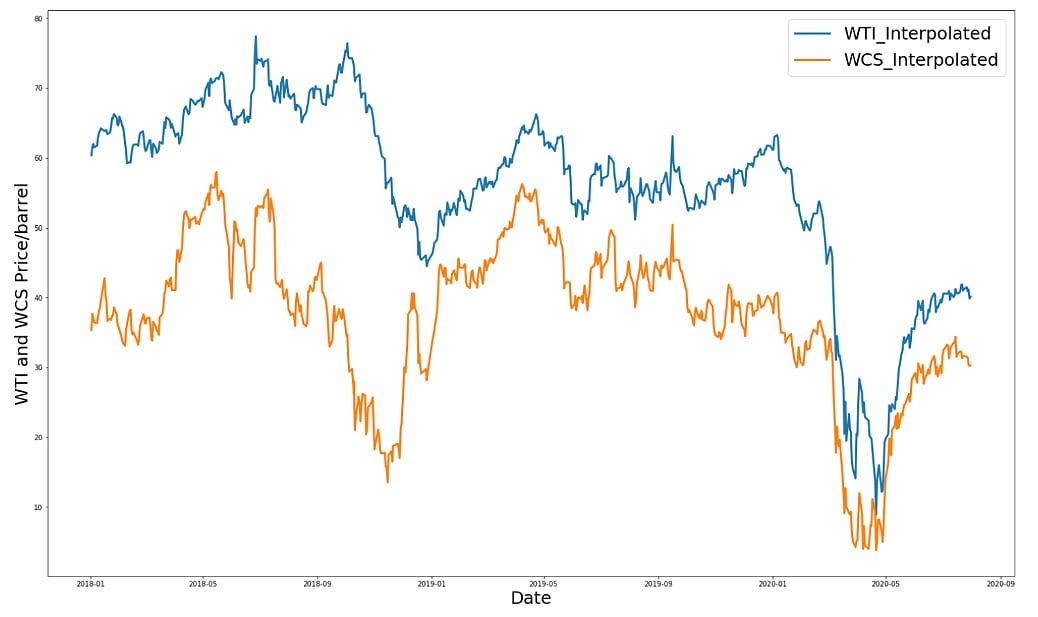
\includegraphics[scale=0.3]{OM-images/price.PNG}
\end{figure}
\end{frame}


\begin{frame}{Introduction (cont.)}
\Large{Global and US oil price benchmarks set the stage for Alberta prices }
    \begin{itemize}
\setlength\itemsep{2em}
    \item \Large{West Texas Intermediate(WTI)}
    \item \Large{West Canada Select (WCS)}
\end{itemize}
\end{frame}

%I highly recommend removing "{Introduction(Cont.)}" from this slide to make as much room as possible for the figure.
\begin{frame}{Introduction(Cont.)}
\centering
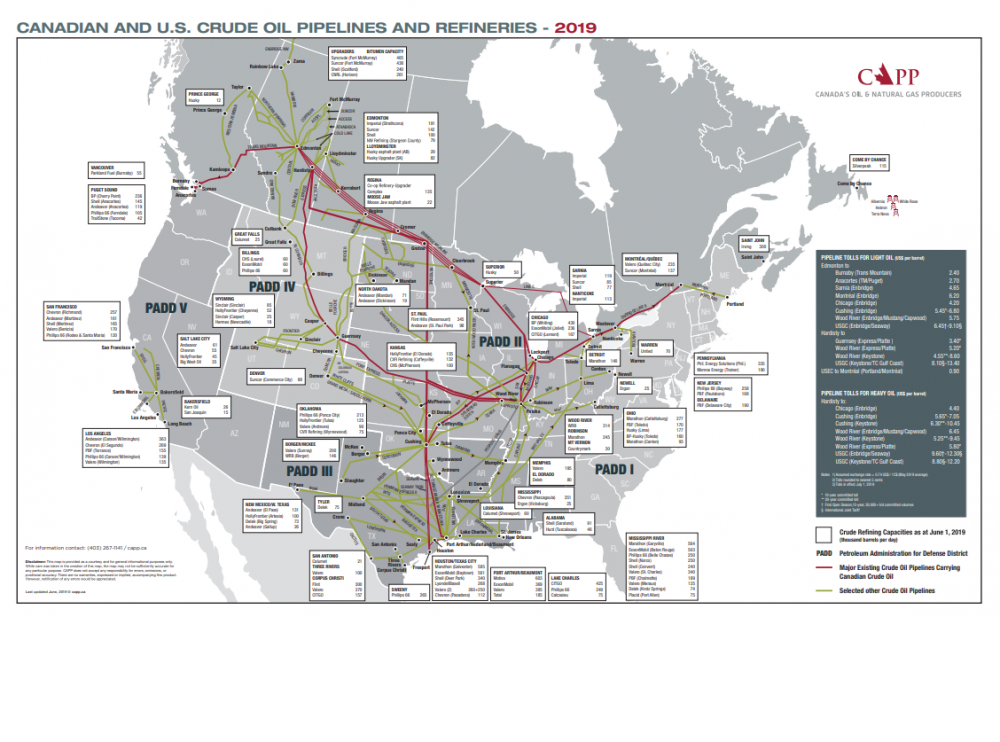
\includegraphics[scale=0.50]{OM-images/piplines.png}
\end{frame}



\begin{frame}{Model - Price decomposition of the spread}
We assume that the WTI--WCS price spread follows the following price decomposition
    \[\lambda^{t} = \rho + \varepsilon^{t} + \omega^{t}\]
where
\begin{enumerate}
    \item $\lambda^{t}$: the WTS--WCS price spread at time $t$;
    \item $\rho$: the transportation cost;
    \item $\varepsilon^{t}$: an equilibrium asset value;
    \item $\omega^{t}$: the congestion surcharge at time $t$.
\end{enumerate}
\end{frame}

\begin{frame}{Model - The neutral band}
\begin{alertblock}{Uniqueness}
{In general, equilibrium prices are NOT unique in a transportation network.}\end{alertblock}
\begin{example}
The price of a bottle of olive oil is \$15 in Vancouver (YVR) and \$20 in Calgary (YYC). It costs \$8 to transport each bottle between YVR and YYC.
\end{example}
Is there arbitrage? 
\end{frame}

\begin{frame}{Model - The neutral band}
\begin{alertblock}{Uniqueness}
{In general, equilibrium prices are NOT unique in a transportation network.}\end{alertblock}
\begin{example}
The price of a bottle of olive oil is \$15 in Vancouver (YVR) and \$20 in Calgary (YYC). It costs \$8 to transport each bottle between YVR and YYC.
\end{example}
Is there arbitrage?

No. The price at YVR in the interval [\$12, \$23] and there will be no arbitrage. We call this the \emph{neutral band}.
\end{frame}
%%%can you please title the slides as the content? for example if you are talking about the Model please title it as Model and then the rest, so as results and conclusion 

%OK - I see what you mean

% Please follow the convention say, "Introduction - Something about the introduction"
% That is, we capitalize Introduction, Model, Result, Conclusion we use a dash and then capitalize the first word after.



\begin{frame}{Model - A one node model}
\begin{align*}
\text{minimize: } &\alpha\\\label{2}
\text{subject to: } &\lambda^t = \rho + \varepsilon^t +\omega^t, \quad \forall t\in\T,\\
&-\alpha\leq\varepsilon^t \leq \alpha,\quad \forall t\in \T\\
&0\leq\omega^t\leq \psi^t M,\quad \forall t\in\T\\
&\varepsilon^t \geq \alpha - (1-\psi^t) M,\quad \forall t\in \T\\
&\sum_t \psi^t \leq \beta T,\\
&\psi^t \in\{0,1\}, \quad \forall t\in \T.
\end{align*}
\end{frame}


\begin{frame}{Model - Mixed integer programming model}
\begin{figure}
%\footnotesize
\begin{equation*}
\begin{split}
\text{minimize: } &\sum_{s\in\S} \alpha_s\\
\text{subject to: } &\lambda_s^t = \rho_s + \varepsilon_s^t +\omega_s^t, \quad \forall s\in\S,~\forall t\in\T,\\
&-\alpha_s\leq\varepsilon_s^t \leq \alpha_s,\\
&0\leq\omega_s^t\leq \psi^t M,\\
&\varepsilon_s^t \geq \alpha_s - (1-\gamma_s^t) M,\\
&\sum_s \gamma_s^t\geq \psi^t,\\
&\sum_t \psi^t \leq \beta T,\\
&\psi^t, \gamma_s^t \in\{0,1\},
\end{split}
\end{equation*}
\end{figure}
\end{frame} 





\begin{frame}{Model - Ornstein--Uhlenbeck Process}
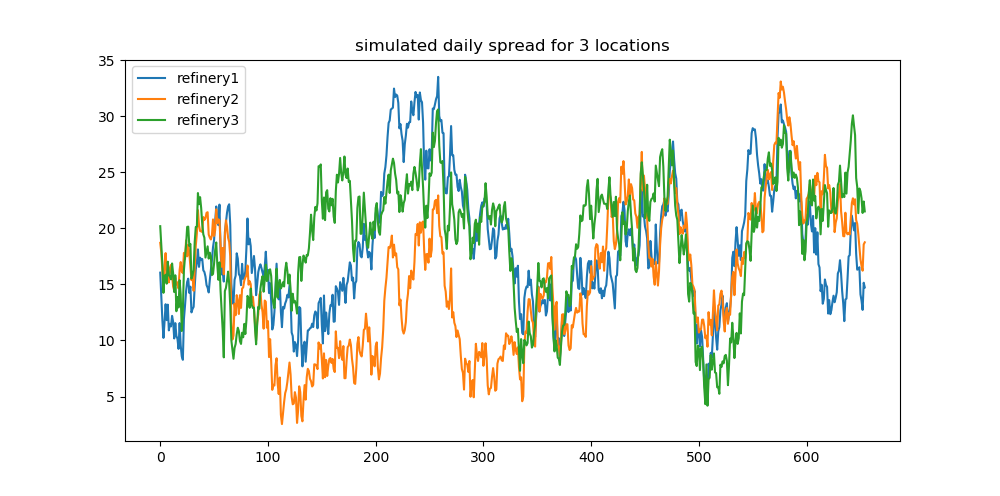
\includegraphics[width=\linewidth]{simulated spread.png}
\end{frame}


\section{Progress}


\begin{frame}{Progress(Cont.)}
\Large{The percentage of the time that congestion happens}
 \begin{figure}
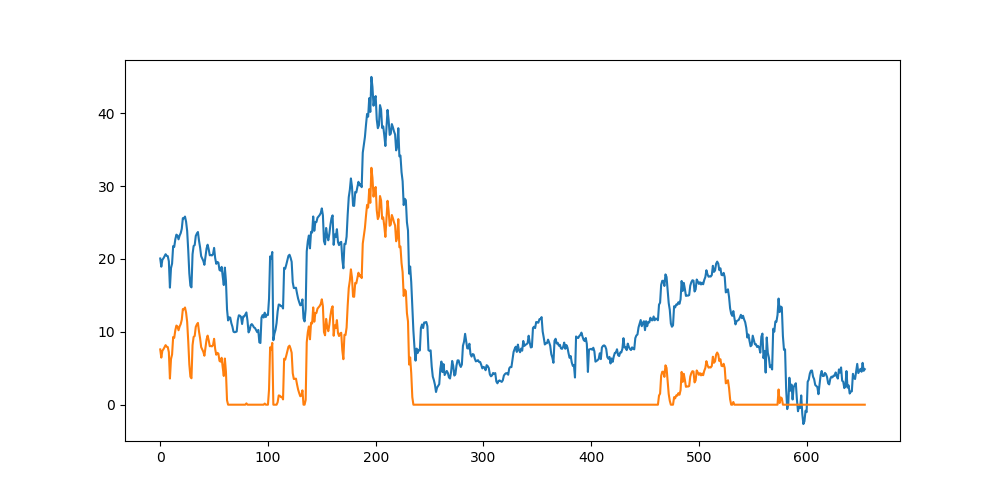
\includegraphics[scale=0.5]{OM-images/betha.png}
\end{figure}
\end{frame}

\begin{frame}{THIS SLIDE FOR THANKS}
    
\end{frame}

\end{document}